\documentclass[border=3pt]{standalone}
% Preâmbulo compartilhado pelos diagramas TikZ da aula 9 de IHR (Robôs na Sociedade)
\usepackage[T1]{fontenc}
\usepackage[utf8]{inputenc}
\usepackage{lmodern}
\usepackage{amsmath}
\usepackage{xcolor}
\usepackage{tikz}
\usetikzlibrary{arrows.meta,angles,quotes,decorations.pathmorphing,decorations.pathreplacing,calc,
                positioning,shapes.geometric,shapes.misc,backgrounds,fit,
                math}

% Paleta (mesma dos SVGs originais)
% Paleta da disciplina de IHR: acento azul (#1A6FB5), cor de destaque do tema.
% (o nome "dblue" é mantido para não alterar todos os diagramas)
\definecolor{dblue}{HTML}{1A6FB5}
\definecolor{dorange}{HTML}{B3541E}
\definecolor{dgreen}{HTML}{4A7C59}
\definecolor{dred}{HTML}{9C4B4B}
\definecolor{dcream}{HTML}{F4F1EA}
\definecolor{dshade}{HTML}{DDD7C9}

% Função gaussiana (não normalizada por padrão de escala visual)
\pgfmathdeclarefunction{gauss}{3}{%
  \pgfmathparse{1/(#3*sqrt(2*pi))*exp(-((#1-#2)^2)/(2*#3^2))}%
}

% Estilos comuns (prefixo d... para não colidir com chaves internas do pgf)
\tikzset{
  >={Stealth[length=2mm]},
  dguide/.style={gray!55, dashed, line width=0.4pt},
  daxis/.style={gray!60, line width=0.7pt, ->},
  dbody/.style={fill=black!3, draw=black!80, line width=1pt},
  dacc/.style={draw=dblue, line width=1pt},
  dlbl/.style={black!55, font=\small},
  dsub/.style={black!45, font=\footnotesize},
  dstate/.style={circle, draw=black!80, fill=dcream, line width=1pt,
                 minimum size=17mm, font=\large, inner sep=1pt},
  dobs/.style={circle, draw=black!80, fill=dshade, line width=1pt,
               minimum size=14mm, font=\large, inner sep=1pt},
  dbox/.style={rounded corners=2pt, draw=black!80, fill=dcream, line width=1pt,
               align=center, inner sep=6pt},
  dop/.style={circle, draw=black!80, fill=white, line width=1pt,
              minimum size=6mm, inner sep=0pt, font=\small},
  dtrans/.style={->, dblue, line width=1pt},
  dmeas/.style={->, dorange, line width=1pt},
  dcurve/.style={line width=1pt, dblue},
  dcurveb/.style={line width=1.4pt, dorange},
}

\begin{document}
\hyphenpenalty=10000 \exhyphenpenalty=10000 \tolerance=9999 \emergencystretch=3em
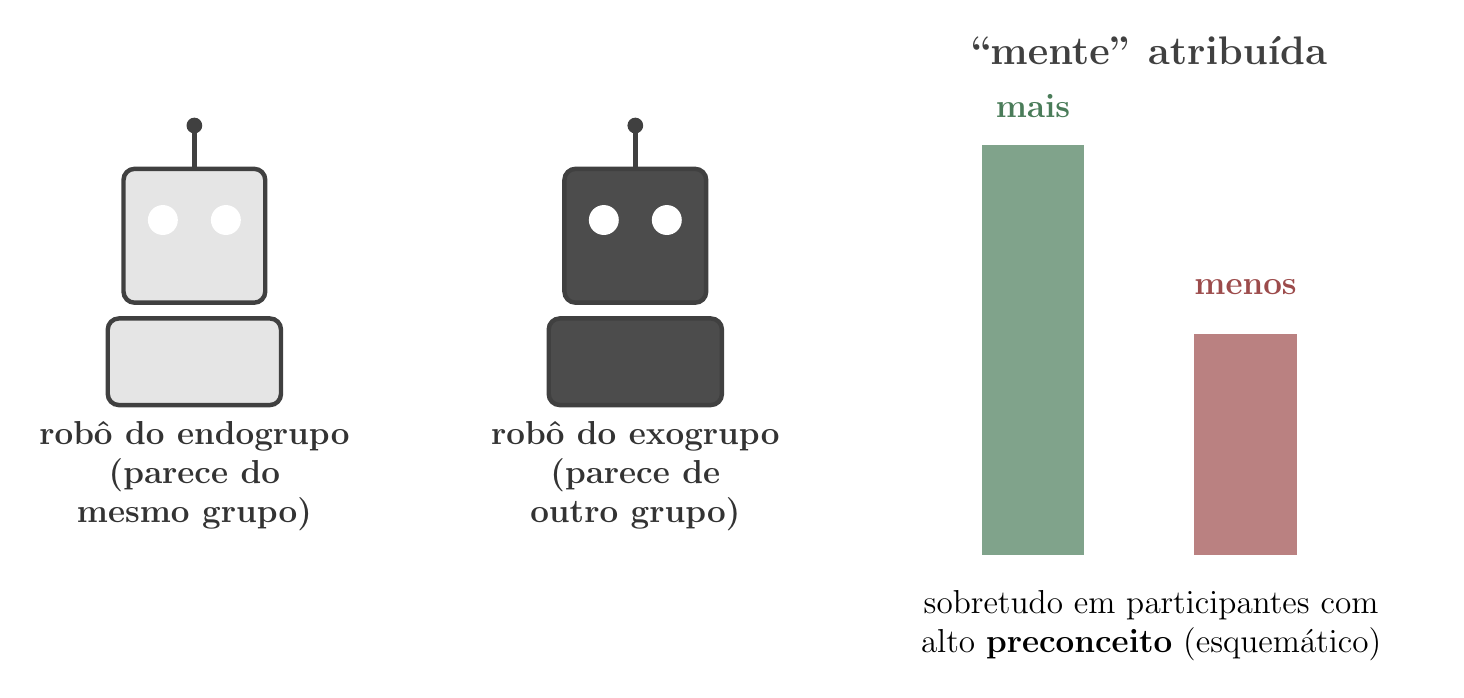
\begin{tikzpicture}[x=1cm,y=1cm]
\newcommand{\rob}[3]{% x, y, fill
  \draw[black!75, fill=#3, line width=1.6pt, rounded corners=4pt] (#1-0.9,#2-0.8) rectangle (#1+0.9,#2+0.9);
  \fill[white] (#1-0.4,#2+0.25) circle (0.19); \fill[white] (#1+0.4,#2+0.25) circle (0.19);
  \draw[black!75, line width=1.6pt] (#1,#2+0.9) -- (#1,#2+1.35); \fill[black!75] (#1,#2+1.45) circle (0.1);
  \draw[black!75, fill=#3, line width=1.6pt, rounded corners=4pt] (#1-1.1,#2-2.1) rectangle (#1+1.1,#2-1.0);}
\rob{2.6}{5.6}{black!10}
\rob{8.2}{5.6}{black!70}
\node[font=\large\bfseries, black!80, text width=4cm, align=center] at (2.6,2.6) {robô do \textbf{endogrupo}\\ (parece do mesmo grupo)};
\node[font=\large\bfseries, black!80, text width=4cm, align=center] at (8.2,2.6) {robô do \textbf{exogrupo}\\ (parece de outro grupo)};
\node[font=\Large\bfseries, black!75] at (14.7,8.0) {``mente'' atribuída};
\fill[dgreen!70] (12.6,1.6) rectangle (13.9,6.8);
\fill[dred!70] (15.3,1.6) rectangle (16.6,4.4);
\node[font=\large\bfseries, dgreen] at (13.25,7.3) {mais};
\node[font=\large\bfseries, dred] at (15.95,5.0) {menos};
\node[font=\large, text width=7cm, align=center] at (14.75,0.7) {sobretudo em participantes com alto \textbf{preconceito} (esquemático)};
\end{tikzpicture}
\end{document}
